\documentclass[12pt]{article}
% Full article preamble (duplicated, no common file)
\usepackage{fontspec}
\usepackage[a4paper,margin=2.5cm,includefoot]{geometry}
\usepackage{polyglossia}
\usepackage{amsmath}
\usepackage{amssymb}
\usepackage{xcolor}
\usepackage{fancyhdr}
\usepackage{graphicx}
\usepackage{listings}
\usepackage[most]{tcolorbox}
\usepackage{pifont}
\usepackage{enumitem}
\usepackage{titlesec}
\usepackage[bottom]{footmisc}
\usepackage{titling}
\usepackage{minted}
\usepackage{etoolbox}
\usepackage{array}
\usepackage{extsizes}

\newfontfamily\emoji{Segoe UI Emoji}

\pagestyle{fancy}

\setmainlanguage[numerals=western]{arabic}
\setotherlanguage{english}
\newfontfamily\arabicfont[Script=Arabic]{Amiri}
\newfontfamily\arabicfonttt[Script=Arabic]{Courier New}

\lstset{
  language=[Sharp]C,
  numbers=left,
  stepnumber=1,
  numbersep=8pt,
  frame=single,
  basicstyle=\ttfamily\small,
  keywordstyle=\color{blue},
  stringstyle=\color{red},
  commentstyle=\color{green!50!black}
}

\newif\ifdetailed
\ifdefined\setdetailed
  \setdetailed
\fi

\newif\ifwithsols
\ifdefined\setwithsols
  \setwithsols
\fi

% unified tcolorboxes for articles
\tcbset{colback=white, colframe=black, fonttitle=\bfseries, boxrule=0.8pt}
\newtcolorbox{boxDef}[1][]{colback=blue!5!white,colframe=blue!75!black,
  title={{\emoji📘} تعريف\ifx\\#1\\\else ~#1\fi :}}
\newtcolorbox{boxExercise}[1][]{colback=cyan!5!white,colframe=cyan!70!black,
  title={{\emoji🧩} تمرين\ifx\\#1\\\else ~#1\fi :}}
\newtcolorbox{boxExample}[1][]{colback=yellow!5!white,colframe=orange!90!black,
  title={{\emoji📝} مثال\ifx\\#1\\\else ~#1\fi :}}
\newtcolorbox{boxNote}[1][]{colback=gray!10!white,colframe=black,
  title={{\emoji✨} ملاحظة\ifx\\#1\\\else ~#1\fi :}}
\newtcolorbox{boxAttention}[1][]{colback=magenta!10!white,colframe=magenta!80!black,
  title={{\emoji🔔} تنبيه\ifx\\#1\\\else ~#1\fi :}}
\newtcolorbox{boxWarning}[1][]{colback=red!5!white,colframe=red!75!black,
  title={{\emoji⚡} ملاحظة هامة\ifx\\#1\\\else ~#1\fi :}}
\newtcolorbox{boxSolution}[1][]{colback=green!5!white,colframe=green!60!black,
  title={{\emoji✅} حل\ifx\\#1\\\else ~#1\fi :}}
\newtcolorbox{boxSymbol}[1][]{colback=purple!5!white,colframe=purple!70!black,
  title={{\emoji🔣} رمز\ifx\\#1\\\else ~#1\fi :}}

\tcbset{simplecode/.style={ colback=gray!5, colframe=black!50, boxrule=0.4pt, arc=2pt, left=4pt,right=4pt,top=4pt,bottom=4pt}}
\newenvironment{boxCode}{\begin{tcolorbox}[simplecode]}{\end{tcolorbox}}

\newcolumntype{C}[1]{>{\centering\arraybackslash}p{#1}}

% redefine spaces after titles
\makeatletter
\renewcommand{\@maketitle}{%
  \begin{center}
    {\huge \bfseries \@title \par}%
    \vskip 0.2em % space between title and author
    {\large \@author \par}%
    % \vskip 0.2em % space between author and date
    % {\normalsize \@date \par}%
  \end{center}
}
\makeatother

\fancyhf{} % clear default
\fancypagestyle{plain}{
  \fancyhf{}
  \fancyhead[L]{مدرسة التسامح الشاملة}
  % \fancyhead[L]{
\includegraphics[height=1cm]{../../../images/logoTasamoh.png}}
  \fancyhead[R]{الأستاذ محمود اغبارية}
  \fancyfoot[C]{\thepage}
}

\fancyhead[L]{مدرسة التسامح الشاملة}
\fancyhead[R]{الأستاذ محمود اغبارية}
\fancyfoot[C]{\thepage}
% \date{\today}

\setcounter{tocdepth}{3} % only section subsection and subsubsection in TOC


% ----------------------


% \begin{document}

% \maketitle

% % \clearpage  % start TOC on a new page
% % \renewcommand{\contentsname}{جدول المحتويات}
% % \tableofcontents
% % \clearpage

% \part*{part 1} % the * prevents numbering
% \section*{مقدمة}
% \subsection*{مثال رياضي}
% \subsubsection*{مثال فرعي}
% \paragraph*{ paragraph 1}
% \subparagraph*{sub paragraph 1}

% \ifdetailed
% \begin{english}
% \begin{minted}{csharp}
% // C# Example
% \end{minted}
% \end{english}
% \fi

% OLD WAY
% \ifdetailed
% \begin{english}
% \begin{lstlisting}
% // C# Example
% \end{lstlisting}
% \end{english}
% \fi

% % 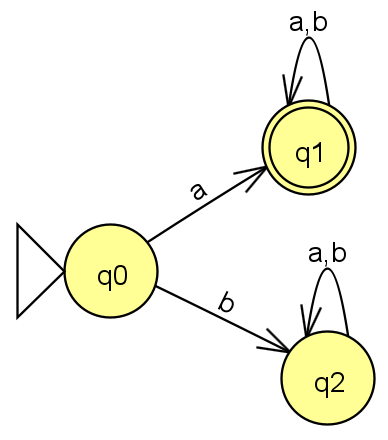
\includegraphics[width=0.2\textwidth]{../../../images/DFAs/ex1_q1.png}



% \vspace{3cm}
% \begin{flushleft}
% أرجو لكم وقتًا ممتعًا.

% الأستاذ محمود اغبارية.
% \end{flushleft}


% \end{document}


\title{أمثلة على العمليات على الكلمات واللغات}

\begin{document}

\maketitle

\renewcommand{\contentsname}{جدول المحتويات}
\tableofcontents
\clearpage

\section{الاتحاد \((L_1 \cup L_2)\)}
\begin{enumerate}
  \item إذا كان \(L_1 = \{a, b\}\) و\(L_2 = \{b, c\}\)
  \ifwithsols
  \begin{boxSolution}
  \(L_1 \cup L_2 = \{a, b, c\}\)
  \end{boxSolution}
  \fi

  \item \(L_1 = \{0, 1\}\)، \(L_2 = \{1, 2\}\)
  \ifwithsols
  \begin{boxSolution}
  \(L_1 \cup L_2 = \{0, 1, 2\}\)
  \end{boxSolution}
  \fi

  \item \(L_1 = \{a, ab\}\)، \(L_2 = \{b, ba\}\)
  \ifwithsols
  \begin{boxSolution}
  \(L_1 \cup L_2 = \{a, ab, b, ba\}\)
  \end{boxSolution}
  \fi

  \item \(L_1 = \{\epsilon, a\}\)، \(L_2 = \{b\}\)
  \ifwithsols
  \begin{boxSolution}
  \(L_1 \cup L_2 = \{\epsilon, a, b\}\)
  \end{boxSolution}
  \fi

  \item \(L_1 = \{a, aa, aaa\}\)، \(L_2 = \{aaa, aaaa\}\)
  \ifwithsols
  \begin{boxSolution}
  \(L_1 \cup L_2 = \{a, aa, aaa, aaaa\}\)
  \end{boxSolution}
  \fi

  \item \(L_1 = \{01, 10\}\)، \(L_2 = \{00, 11\}\)
  \ifwithsols
  \begin{boxSolution}
  \(L_1 \cup L_2 = \{00, 01, 10, 11\}\)
  \end{boxSolution}
  \fi

  \item \(L_1 = \{x, y\}\)، \(L_2 = \{y, z\}\)
  \ifwithsols
  \begin{boxSolution}
  \(L_1 \cup L_2 = \{x, y, z\}\)
  \end{boxSolution}
  \fi

  \item \(L_1 = \{ab, ba\}\)، \(L_2 = \{a, b\}\)
  \ifwithsols
  \begin{boxSolution}
  \(L_1 \cup L_2 = \{a, b, ab, ba\}\)
  \end{boxSolution}
  \fi

  \item \(L_1 = \{a, bb\}\)، \(L_2 = \{bb, c\}\)
  \ifwithsols
  \begin{boxSolution}
  \(L_1 \cup L_2 = \{a, bb, c\}\)
  \end{boxSolution}
  \fi

  \item \(L_1 = \{0, 00\}\)، \(L_2 = \{1, 11\}\)
  \ifwithsols
  \begin{boxSolution}
  \(L_1 \cup L_2 = \{0, 00, 1, 11\}\)
  \end{boxSolution}
  \fi
  \item \(L_1 = \emptyset,\; L_2 = \{a\}\)
  \ifwithsols
  \begin{boxSolution}
  \(L_1 \cup L_2 = \{a\}\)
  \end{boxSolution}
  \fi

  \item \(L_1 = \{b\},\; L_2 = \emptyset\)
  \ifwithsols
  \begin{boxSolution}
  \(L_1 \cup L_2 = \{b\}\)
  \end{boxSolution}
  \fi

  \item \(L_1 = \emptyset,\; L_2 = \emptyset\)
  \ifwithsols
  \begin{boxSolution}
  \(L_1 \cup L_2 = \emptyset\)
  \end{boxSolution}
  \fi

  \item \(L_1 = \{\epsilon\},\; L_2 = \{a\}\)
  \ifwithsols
  \begin{boxSolution}
  \(L_1 \cup L_2 = \{\epsilon, a\}\)
  \end{boxSolution}
  \fi

  \item \(L_1 = \{\epsilon\},\; L_2 = \emptyset\)
  \ifwithsols
  \begin{boxSolution}
  \(L_1 \cup L_2 = \{\epsilon\}\)
  \end{boxSolution}
  \fi
\end{enumerate}


\clearpage
\section{التقاطع \((L_1 \cap L_2)\)}
\begin{enumerate}
  \item \(L_1 = \{a, b\}\)، \(L_2 = \{b, c\}\)
  \ifwithsols
  \begin{boxSolution}
  \(L_1 \cap L_2 = \{b\}\)
  \end{boxSolution}
  \fi

  \item \(L_1 = \{0, 01, 10\}\)، \(L_2 = \{01, 11\}\)
  \ifwithsols
  \begin{boxSolution}
  \(L_1 \cap L_2 = \{01\}\)
  \end{boxSolution}
  \fi

  \item \(L_1 = \{a, ab, abc\}\)، \(L_2 = \{ab, ac\}\)
  \ifwithsols
  \begin{boxSolution}
  \(L_1 \cap L_2 = \{ab\}\)
  \end{boxSolution}
  \fi

  \item \(L_1 = \{x, xy\}\)، \(L_2 = \{y, xy\}\)
  \ifwithsols
  \begin{boxSolution}
  \(L_1 \cap L_2 = \{xy\}\)
  \end{boxSolution}
  \fi

  \item \(L_1 = \{aa, bb\}\)، \(L_2 = \{bb, cc\}\)
  \ifwithsols
  \begin{boxSolution}
  \(L_1 \cap L_2 = \{bb\}\)
  \end{boxSolution}
  \fi

  \item \(L_1 = \{\epsilon, a, b\}\)، \(L_2 = \{b, c\}\)
  \ifwithsols
  \begin{boxSolution}
  \(L_1 \cap L_2 = \{b\}\)
  \end{boxSolution}
  \fi

  \item \(L_1 = \{10, 01\}\)، \(L_2 = \{01, 11\}\)
  \ifwithsols
  \begin{boxSolution}
  \(L_1 \cap L_2 = \{01\}\)
  \end{boxSolution}
  \fi

  \item \(L_1 = \{ab, ba, aa\}\)، \(L_2 = \{ba, aa, bb\}\)
  \ifwithsols
  \begin{boxSolution}
  \(L_1 \cap L_2 = \{ba, aa\}\)
  \end{boxSolution}
  \fi

  \item \(L_1 = \{a, b, c\}\)، \(L_2 = \{c, d, e\}\)
  \ifwithsols
  \begin{boxSolution}
  \(L_1 \cap L_2 = \{c\}\)
  \end{boxSolution}
  \fi

  \item \(L_1 = \{a, aa\}\)، \(L_2 = \{aa, aaa\}\)
  \ifwithsols
  \begin{boxSolution}
  \(L_1 \cap L_2 = \{aa\}\)
  \end{boxSolution}
  \fi

  \item \(L_1 = \emptyset,\; L_2 = \{a\}\)
  \ifwithsols
  \begin{boxSolution}
  \(L_1 \cap L_2 = \emptyset\)
  \end{boxSolution}
  \fi

  \item \(L_1 = \{b\},\; L_2 = \emptyset\)
  \ifwithsols
  \begin{boxSolution}
  \(L_1 \cap L_2 = \emptyset\)
  \end{boxSolution}
  \fi

  \item \(L_1 = \emptyset,\; L_2 = \emptyset\)
  \ifwithsols
  \begin{boxSolution}
  \(L_1 \cap L_2 = \emptyset\)
  \end{boxSolution}
  \fi

  \item \(L_1 = \{\epsilon\},\; L_2 = \{a, b\}\)
  \ifwithsols
  \begin{boxSolution}
  \(L_1 \cap L_2 = \emptyset\)
  \end{boxSolution}
  \fi

  \item \(L_1 = \{\epsilon, a\},\; L_2 = \{\epsilon\}\)
  \ifwithsols
  \begin{boxSolution}
  \(L_1 \cap L_2 = \{\epsilon\}\)
  \end{boxSolution}
  \fi
\end{enumerate}


\clearpage
\section{القوة لعدد \((L^n)\)}
\begin{enumerate}
  \item \(L = \{a\},\; n=3\)
  \ifwithsols
  \begin{boxSolution}
  \(L^3 = \{aaa\}\)
  \end{boxSolution}
  \fi

  \item \(L = \{ab\},\; n=2\)
  \ifwithsols
  \begin{boxSolution}
  \(L^2 = \{abab\}\)
  \end{boxSolution}
  \fi

  \item \(L = \{0,1\},\; n=2\)
  \ifwithsols
  \begin{boxSolution}
  \(L^2 = \{00, 01, 10, 11\}\)
  \end{boxSolution}
  \fi

  \item \(L = \{a,b\},\; n=3\)
  \ifwithsols
  \begin{boxSolution}
  كل الكلمات من الطول 3 من الحروف \(a,b\):
  \(L^3 = \{aaa, aab, aba, abb, baa, bab, bba, bbb\}\)
  \end{boxSolution}
  \fi

  \item \(L = \{x\},\; n=0\)
  \ifwithsols
  \begin{boxSolution}
  \(L^0 = \{\epsilon\}\)
  \end{boxSolution}
  \fi

  \item \(L = \{\epsilon, a\},\; n=2\)
  \ifwithsols
  \begin{boxSolution}
  \(L^2 = \{\epsilon, a, aa\}\)
  \end{boxSolution}
  \fi

  \item \(L = \{a, ab\},\; n=2\)
  \ifwithsols
  \begin{boxSolution}
  \(L^2 = \{aa, aab, aba, abab\}\)
  \end{boxSolution}
  \fi

  \item \(L = \{01,10\},\; n=2\)
  \ifwithsols
  \begin{boxSolution}
  \(L^2 = \{0101, 0110, 1001, 1010\}\)
  \end{boxSolution}
  \fi

  \item \(L = \{p,q\},\; n=3\)
  \ifwithsols
  \begin{boxSolution}
  \(L^3\) هي جميع الكلمات من الطول 3 من \(p,q\): \(L^3 = \{ ppp, ppq, pqp, pqq, qpp, qpq, qqp, qqq \}\)
  \end{boxSolution}
  \fi

  \item \(L = \{aa, bb\},\; n=2\)
  \ifwithsols
  \begin{boxSolution}
  \(L^2 = \{aaaa, aabb, bbaa, bbbb\}\)
  \end{boxSolution}
  \fi

  \item \(L=\emptyset,\; n=2\)
  \ifwithsols
  \begin{boxSolution}
  \(\emptyset^2 = \emptyset\) (لأنّه لا توجد كلمة يمكن أخذها مرتين).
  \end{boxSolution}
  \fi

  \item \(L=\emptyset,\; n=0\)
  \ifwithsols
  \begin{boxSolution}
  عادةً \(L^0 = \{\epsilon\}\) لأي لغة \(L\)، بما في ذلك \(\emptyset\). إذن \(\emptyset^0 = \{\epsilon\}\).
  \end{boxSolution}
  \fi

  \item \(L=\emptyset,\; n=1\)
  \ifwithsols
  \begin{boxSolution}
  \(\emptyset^1 = \emptyset\).
  \end{boxSolution}
  \fi

  \item \(L=\{\epsilon\},\; n=5\)
  \ifwithsols
  \begin{boxSolution}
  \(\{\epsilon\}^5 = \{\epsilon\}\) (لأن \(\epsilon\epsilon...\epsilon = \epsilon\)).
  \end{boxSolution}
  \fi

  \item \(L=\{\epsilon\},\; n=0\)
  \ifwithsols
  \begin{boxSolution}
  \(\{\epsilon\}^0 = \{\epsilon\}\) (حسب التعريف العام).
  \end{boxSolution}
  \fi
\end{enumerate}


\clearpage
\section{القوة للنجمة \((L^*)\)}
\begin{enumerate}
  \item \(L = \{a\}\)
  \ifwithsols
  \begin{boxSolution}
  \(L^* = \{\epsilon, a, aa, aaa, \dots\}\)
  \end{boxSolution}
  \fi
  \item \(L = \{0,1\}\)
  \ifwithsols
  \begin{boxSolution}
  جميع السلاسل من 0 و1:
  \(\{\epsilon, 0, 1, 00, 01, 10, 11, \dots\}\)
  \end{boxSolution}
  \fi
  \item \(L = \{ab\}\)
  \ifwithsols
  \begin{boxSolution}
  \(L^* = \{\epsilon, ab, abab, ababab, \dots\}\)
  \end{boxSolution}
  \fi
  \item \(L = \{a,b\}\)
  \ifwithsols
  \begin{boxSolution}
  جميع الكلمات من \(a,b\) بطول أي عدد
  \end{boxSolution}
  \fi
  \item \(L = \{x\}\)
  \ifwithsols
  \begin{boxSolution}
  \(\{\epsilon, x, xx, xxx, \dots\}\)
  \end{boxSolution}
  \fi
  \item \(L = \{aa\}\)
  \ifwithsols
  \begin{boxSolution}
  كل الكلمات المكونة من عدد زوجي من الـ \(a\) يشمل الكلمة الفارغة. \\
  \(\{\epsilon, aa, aaaa, aaaaaa, \dots\}\)
  \end{boxSolution}
  \fi
  \item \(L = \{ab, ba\}\)
  \ifwithsols
  \begin{boxSolution}
  جميع التراكيب من ab وba بطول غير محدود \\
  \( L^* = \{\epsilon, ab, ba, abab, abba, baba, baab, \dots \} \)
  \end{boxSolution}
  \fi
  \item \(L = \{a, \epsilon\}\)
  \ifwithsols
  \begin{boxSolution}
  \(L^* = \{\epsilon, a, aa, aaa, \dots\}\) \\
\end{boxSolution}
\begin{boxAttention}
    لاحظ أنّ: \( \{ \epsilon, a \}^* = \{ a \}^* \)
\end{boxAttention}
  \fi
  \item \(L = \{01\}\)
  \ifwithsols
  \begin{boxSolution}
  \(\{\epsilon, 01, 0101, 010101, \dots\}\) \\
كل الكلمات المكون من $0$ ثم يتبعها $1$ مباشرة.
  \end{boxSolution}
  \fi
  \item \(L = \{a,b,c\}\)
  \ifwithsols
  \begin{boxSolution}
  جميع الكلمات الممكنة من الحروف \(a,b,c\)
  \end{boxSolution}
  \fi

  \item \(L=\emptyset\)
  \ifwithsols
  \begin{boxSolution}
  \(\emptyset^* = \{\epsilon\}\) (النجمة دائمًا تحتوي على \(\epsilon\)).
  \end{boxSolution}
  \fi

  \item \(L=\{\epsilon\}\)
  \ifwithsols
  \begin{boxSolution}
  \(\{\epsilon\}^* = \{\epsilon\}\) لأنّ تكرار \(\epsilon\) يعطي دائمًا \(\epsilon\).
  \end{boxSolution}
  \fi
\end{enumerate}


\clearpage
\section{القوة للزائد \((L^+)\)}
\begin{enumerate}
  \item \(L = \{a\}\)
  \ifwithsols
  \begin{boxSolution}
  \(L^+ = \{a, aa, aaa, \dots\}\)
  \end{boxSolution}
  \fi
  \item \(L = \{0,1\}\)
  \ifwithsols
  \begin{boxSolution}
  جميع الكلمات غير الفارغة من 0 و1
  \end{boxSolution}
  \fi
  \item \(L = \{ab\}\)
  \ifwithsols
  \begin{boxSolution}
  \(L^+ = \{ab, abab, ababab, \dots\}\)
  \end{boxSolution}
  \fi
  \item \(L = \{a,b\}\)
  \ifwithsols
  \begin{boxSolution}
  جميع الكلمات من \(a,b\) ذات طول أكبر من صفر
  \end{boxSolution}
  \fi
  \item \(L = \{x\}\)
  \ifwithsols
  \begin{boxSolution}
  \(\{x, xx, xxx, \dots\}\)
  \end{boxSolution}
  \fi
  \item \(L = \{aa\}\)
  \ifwithsols
  \begin{boxSolution}
  \(\{aa, aaaa, aaaaaa, \dots\}\)
  \end{boxSolution}
  \fi
  \item \(L = \{ab, ba\}\)
  \ifwithsols
  \begin{boxSolution}
  كل التراكيب الممكنة من ab وba على الأقل مرة واحدة \\
  \( L^+ = \{ ab, ba, abab, baba, abba, baab, \dots \} \)
  \end{boxSolution}
  \fi
  \item \(L = \{a, \epsilon\}\)
  \ifwithsols
  \begin{boxSolution}
  \(L^+ = \{a, aa, aaa, \dots\}\)
  \end{boxSolution}
  \fi
  \item \(L = \{01\}\)
  \ifwithsols
  \begin{boxSolution}
  \(\{01, 0101, 010101, \dots\}\)
  \end{boxSolution}
  \fi
  \item \(L = \{a,b,c\}\)
  \ifwithsols
  \begin{boxSolution}
  جميع الكلمات من \(a,b,c\) بطول $1 \leq$
  \end{boxSolution}
  \fi

  \item \(L=\emptyset\)
  \ifwithsols
  \begin{boxSolution}
  \(\emptyset^+ = \emptyset\) (لأنّ النجمة تعطي \(\{\epsilon\}\) لكن الزائد يتطلب تكرارًا ≥1، فلا كلمات).
  \end{boxSolution}
  \fi

  \item \(L=\{\epsilon\}\)
  \ifwithsols
  \begin{boxSolution}
  \(\{\epsilon\}^+ = \{\epsilon\}\).
  \end{boxSolution}
  \fi
\end{enumerate}


\clearpage
\section{ضرب كلمات (إلصاق)}
\begin{enumerate}
  \item \(x = a,\; y = b\)
  \ifwithsols
  \begin{boxSolution}
  \(xy = ab \quad;\quad yx = ba \)
  \end{boxSolution}
  \fi

  \item \(x = ab,\; y = c\)
  \ifwithsols
  \begin{boxSolution}
  \(xy = abc \quad;\quad yx = cab \)
  \end{boxSolution}
  \fi

  \item \(x = a,\; y = \epsilon\)
  \ifwithsols
  \begin{boxSolution}
  \(xy = a \quad;\quad yx = a\)
  \end{boxSolution}
  \fi

  \item \(x = \epsilon,\; y = b\)
  \ifwithsols
  \begin{boxSolution}
  \(xy = b \quad;\quad yx = b\)
  \end{boxSolution}
  \fi

  \item \(x = \epsilon,\; y = \epsilon \)
  \ifwithsols
  \begin{boxSolution}
  \(xy = \epsilon \quad;\quad yx = \epsilon \)
  \end{boxSolution}
  \fi

  \item \(x = 01,\; y = 10\)
  \ifwithsols
  \begin{boxSolution}
  \(xy = 0110 \quad;\quad yx = 1001\)
  \end{boxSolution}
  \fi

  \item \(x = ab,\; y = ba\)
  \ifwithsols
  \begin{boxSolution}
  \(xy = abba \quad;\quad yx = baab\)
  \end{boxSolution}
  \fi

  \item \(x = x,\; y = yx\)
  \ifwithsols
  \begin{boxSolution}
  \(xy = xyx \quad;\quad yx = yxx \)
  \end{boxSolution}
  \fi

  \item \(x = a,\; y = aa\)
  \ifwithsols
  \begin{boxSolution}
  \(xy = aaa \quad;\quad yx = aaa\)
  \end{boxSolution}
  \fi

  \item \(x = 0,\; y = 111\)
  \ifwithsols
  \begin{boxSolution}
  \(xy = 0111 \quad;\quad yx = 1110\)
  \end{boxSolution}
  \fi

  \item \(x = ab,\; y = ab\)
  \ifwithsols
  \begin{boxSolution}
  \(xy = abab \quad;\quad yx = abab\)
  \end{boxSolution}
  \fi

  \item \(x=\epsilon,\; y=a\)
  \ifwithsols
  \begin{boxSolution}
  \(xy = \epsilon a = a\).
  \end{boxSolution}
  \fi

  \item \(x=a,\; y=\epsilon\)
  \ifwithsols
  \begin{boxSolution}
  \(xy = a\epsilon = a\).
  \end{boxSolution}
  \fi

  \item \(x=\epsilon,\; y=\epsilon\)
  \ifwithsols
  \begin{boxSolution}
  \(xy = \epsilon\).
  \end{boxSolution}
  \fi
\end{enumerate}


\clearpage
\section{ضرب لغات \((L_1 L_2)\)}
\begin{enumerate}
  \item \(L_1 = \{a\},\; L_2 = \{b\}\)
  \ifwithsols
  \begin{boxSolution}
  \(L_1L_2 = \{ab\} \quad;\quad L_2L_1 = \{ ba \} \)
  \end{boxSolution}
  \fi

  \item \(L_1 = \{a,b\},\; L_2 = \{c\}\)
  \ifwithsols
  \begin{boxSolution}
  \(L_1L_2 = \{ac, bc\} \quad;\quad L_2L_1 = \{ ca, cb \} \)
  \end{boxSolution}
  \fi

  \item \(L_1 = \{0,1\},\; L_2 = \{0\}\)
  \ifwithsols
  \begin{boxSolution}
  \(L_1L_2 = \{00,10\} \quad;\quad L_2L_1 = \{ 00, 01\} \)
  \end{boxSolution}
  \fi

  \item \(L_1 = \{a\},\; L_2 = \{b,c\}\)
  \ifwithsols
  \begin{boxSolution}
  \(L_1L_2 = \{ab, ac\} \quad;\quad L_2L_1 = \{ba, ca\} \)
  \end{boxSolution}
  \fi

  \item \(L_1 = \{x,y\},\; L_2 = \{x\}\)
  \ifwithsols
  \begin{boxSolution}
  \(L_1L_2 = \{xx, yx\} \quad;\quad L_2L_1 = \{xx, xy\} \)
  \end{boxSolution}
  \fi

  \item \(L_1 = \{a,b\},\; L_2 = \{a,b\}\)
  \ifwithsols
  \begin{boxSolution}
  \(L_1L_2 = \{aa, ab, ba, bb\} \quad;\quad L_2L_1 = \{aa, ab, ba, bb\} \)
  \end{boxSolution}
  \fi

  \item \(L_1 = \{a\},\; L_2 = \{\epsilon, b\}\)
  \ifwithsols
  \begin{boxSolution}
  \(L_1L_2 = \{a, ab\} \quad;\quad L_2L_1 = \{a, ba \} \)
  \end{boxSolution}
  \fi

  \item \(L_1 = \{\epsilon, a\},\; L_2 = \{\epsilon, b\}\)
  \ifwithsols
  \begin{boxSolution}
  \(L_1L_2 = \{\epsilon, a, b, ab\} \quad;\quad L_2L_1 = \{\epsilon, a, b, ba \} \)
  \end{boxSolution}
  \fi

  \item \(L_1 = \{01\},\; L_2 = \{1,0\}\)
  \ifwithsols
  \begin{boxSolution}
  \(L_1L_2 = \{011, 010\} \quad;\quad L_2L_1 = \{ 101, 001 \} \)
  \end{boxSolution}
  \fi

  \item \(L_1 = \{ab, ba\},\; L_2 = \{a\}\)
  \ifwithsols
  \begin{boxSolution}
  \(L_1L_2 = \{aba, baa\} \quad;\quad L_2L_1 = \{ aab, aba\} \)
  \end{boxSolution}
  \fi

  \item \(L_1 = \{\epsilon, a\},\; L_2 = \{b\}\)
  \ifwithsols
  \begin{boxSolution}
  \(L_1L_2 = \{b, ab\} \quad;\quad L_2L_1 = \{b, ba\} \)
  \end{boxSolution}
  \fi

  \item \(L_1=\emptyset,\; L_2=\{a\}\)
  \ifwithsols
  \begin{boxSolution}
  \(L_1L_2 = \emptyset\) (لا توجد كلمة من \(L_1\) لتلصقها مع كلمات \(L_2\)).
  \end{boxSolution}
  \fi

  \item \(L_1=\{a\},\; L_2=\emptyset\)
  \ifwithsols
  \begin{boxSolution}
  \(L_1L_2 = \emptyset\).
  \end{boxSolution}
  \fi

  \item \(L_1=\emptyset,\; L_2=\emptyset\)
  \ifwithsols
  \begin{boxSolution}
  \(L_1L_2 = \emptyset\).
  \end{boxSolution}
  \fi

  \item \(L_1=\{\epsilon\},\; L_2=\{a, b\}\)
  \ifwithsols
  \begin{boxSolution}
  \(L_1L_2 = \{a, b\}\) (لأن \(\epsilon a = a\) و \(\epsilon b = b\)).
  \end{boxSolution}
  \fi

  \item \(L_1=\{a, b\},\; L_2=\{\epsilon\}\)
  \ifwithsols
  \begin{boxSolution}
  \(L_1L_2 = \{a, b\}\) (لأن \(a\epsilon = a\) و \(b\epsilon = b\)).
  \end{boxSolution}
  \fi

  \item \(L_1=\{\epsilon\},\; L_2=\emptyset\)
  \ifwithsols
  \begin{boxSolution}
  \(L_1L_2 = \emptyset\) (لأنه لا توجد كلمات في \(L_2\) لنلصقها مع \(\epsilon\)).
  \end{boxSolution}
  \fi
\end{enumerate}


\clearpage
\section{طول كلمة}
\begin{enumerate}
  \item \(w = a\)
  \ifwithsols
  \begin{boxSolution}
  \(|w| = 1\)
  \end{boxSolution}
  \fi

  \item \(w = ab\)
  \ifwithsols
  \begin{boxSolution}
  \(|w| = 2\)
  \end{boxSolution}
  \fi

  \item \(w = 0101\)
  \ifwithsols
  \begin{boxSolution}
  \(|w| = 4\)
  \end{boxSolution}
  \fi

  \item \(w = \epsilon\)
  \ifwithsols
  \begin{boxSolution}
  \(|w| = 0\)
  \end{boxSolution}
  \fi

  \item \(w = abcde\)
  \ifwithsols
  \begin{boxSolution}
  \(|w| = 5\)
  \end{boxSolution}
  \fi

  \item \(w = xxxy\)
  \ifwithsols
  \begin{boxSolution}
  \(|w| = 4\)
  \end{boxSolution}
  \fi

  \item \(w = 111\)
  \ifwithsols
  \begin{boxSolution}
  \(|w| = 3\)
  \end{boxSolution}
  \fi

  \item \(w = abba\)
  \ifwithsols
  \begin{boxSolution}
  \(|w| = 4\)
  \end{boxSolution}
  \fi

  \item \(w = xyxyx\)
  \ifwithsols
  \begin{boxSolution}
  \(|w| = 5\)
  \end{boxSolution}
  \fi

  \item \(w = 0\)
  \ifwithsols
  \begin{boxSolution}
  \(|w| = 1\)
  \end{boxSolution}
  \fi

  \item \(w=\epsilon\)
  \ifwithsols
  \begin{boxSolution}
  \(|\epsilon| = 0\).
  \end{boxSolution}
  \fi
\end{enumerate}


\clearpage
\section{أمثلة على حساب $\#_1(w)$ و $\#_0(w)$}

\begin{enumerate}

\item احسب $\#_1(\epsilon)$
\ifwithsols
\begin{boxSolution}
$\#_1(\epsilon) = 0 \quad;\quad \#_0(\epsilon) = 0$
\end{boxSolution}
\fi

\item احسب $\#_1(0)$
\ifwithsols
\begin{boxSolution}
$\#_1(0) = 0 \quad;\quad \#_0(0) = 1$
\end{boxSolution}
\fi

\item احسب $\#_1(1)$
\ifwithsols
\begin{boxSolution}
$\#_1(1) = 1 \quad;\quad \#_0(1) = 0$
\end{boxSolution}
\fi

\item احسب $\#_1(10)$
\ifwithsols
\begin{boxSolution}
$\#_1(10) = 1 \quad;\quad \#_0(10) = 1$
\end{boxSolution}
\fi

\item احسب $\#_1(01)$
\ifwithsols
\begin{boxSolution}
$\#_1(01) = 1 \quad;\quad \#_0(01) = 1$
\end{boxSolution}
\fi

\item احسب $\#_1(110)$
\ifwithsols
\begin{boxSolution}
$\#_1(110) = 2 \quad;\quad \#_0(110) = 1$
\end{boxSolution}
\fi

\item احسب $\#_1(1011)$
\ifwithsols
\begin{boxSolution}
$\#_1(1011) = 3 \quad;\quad \#_0(1011) = 1$
\end{boxSolution}
\fi

\item احسب $\#_1(0000)$
\ifwithsols
\begin{boxSolution}
$\#_1(0000) = 0 \quad;\quad \#_0(0000) = 4$
\end{boxSolution}
\fi

\item احسب $\#_1(11111)$
\ifwithsols
\begin{boxSolution}
$\#_1(11111) = 5 \quad;\quad \#_0(11111) = 0$
\end{boxSolution}
\fi

\item احسب $\#_1(101010)$
\ifwithsols
\begin{boxSolution}
$\#_1(101010) = 3 \quad;\quad \#_0(101010) = 3$
\end{boxSolution}
\fi

\end{enumerate}

\end{document}